\documentclass[a4paper]{article}
\usepackage{parskip}
\usepackage{lipsum}

\def\nterm {Spring}
\def\nyear {2025}
\def\ncourse {Introduction to Functional Analysis}

\makeatletter
\ifx \nauthor\undefined
  \def\nauthor{Runqiu Ye}
\else
\fi

\author{Notes taken by \nauthor\vspace{5pt}\\ 
Carnegie Mellon University}
\date{\nterm\ \nyear}

\usepackage{alltt}
\usepackage{amsfonts}
\usepackage{amsmath}
\usepackage{amssymb}
\usepackage{amsthm}
\usepackage{booktabs}
\usepackage{caption}
\usepackage{enumitem}
\usepackage{fancyhdr}
\usepackage{graphicx}
\usepackage{mathdots}
\usepackage{mathtools}
\usepackage{microtype}
\usepackage{multirow}
\usepackage{pdflscape}
\usepackage{pgfplots}
\usepackage{siunitx}
\usepackage{slashed}
\usepackage{tabularx}
\usepackage{tikz}
\usepackage{tkz-euclide}
\usepackage[normalem]{ulem}
\usepackage[all]{xy}
\usepackage{imakeidx}
\usepackage[includehead,includefoot, heightrounded,  left=1.0in, top=1.6cm, bottom=2.4cm, right=1.0in]{geometry}
\usepackage{mathrsfs}

\makeindex[intoc, title=Index]
\indexsetup{othercode={\lhead{\emph{Index}}}}

\ifx \nextra \undefined
  \usepackage[pdftex,
    hidelinks,
    pdfauthor={Dexter Chua},
    pdfsubject={\ncourse},
    pdftitle={\ncourse},
  pdfkeywords={Cambridge Mathematics Maths Math \nterm\ \nyear\ \ncourse}]{hyperref}
  \title{\ncourse}
\else
  \usepackage[pdftex,
    hidelinks,
    pdfauthor={Dexter Chua},
    pdfsubject={Cambridge Maths Notes: \ncourse\ (\nextra)},
    pdftitle={\ncourse\ (\nextra)},
  pdfkeywords={Cambridge Mathematics Maths Math \nterm\ \nyear\ \ncourse\ \nextra}]{hyperref}

  \title{\ncourse \\ {\Large \nextra}}
  \renewcommand\printindex{}
\fi

\pgfplotsset{compat=1.12}

\pagestyle{fancyplain}
\ifx \ncoursehead \undefined
\def\ncoursehead{\ncourse}
\fi

\lhead{\emph{\nouppercase{\leftmark}}}
\ifx \nextra \undefined
  \rhead{
    \ifnum\thepage=1
    \else
      \ncoursehead
    \fi}
\else
  \rhead{
    \ifnum\thepage=1
    \else
      \ncoursehead \ (\nextra)
    \fi}
\fi
\usetikzlibrary{arrows.meta}
\usetikzlibrary{decorations.markings}
\usetikzlibrary{decorations.pathmorphing}
\usetikzlibrary{positioning}
\usetikzlibrary{fadings}
\usetikzlibrary{intersections}
\usetikzlibrary{cd}

\newcommand*{\Cdot}{{\raisebox{-0.25ex}{\scalebox{1.5}{$\cdot$}}}}
\newcommand {\pd}[2][ ]{
  \ifx #1 { }
    \frac{\partial}{\partial #2}
  \else
    \frac{\partial^{#1}}{\partial #2^{#1}}
  \fi
}
\ifx \nhtml \undefined
\else
  \renewcommand\printindex{}
  \DisableLigatures[f]{family = *}
  \let\Contentsline\contentsline
  \renewcommand\contentsline[3]{\Contentsline{#1}{#2}{}}
  \renewcommand{\@dotsep}{10000}
  \newlength\currentparindent
  \setlength\currentparindent\parindent

  \newcommand\@minipagerestore{\setlength{\parindent}{\currentparindent}}
  \usepackage[active,tightpage,pdftex]{preview}
  \renewcommand{\PreviewBorder}{0.1cm}

  \newenvironment{stretchpage}%
  {\begin{preview}\begin{minipage}{\hsize}}%
    {\end{minipage}\end{preview}}
  \AtBeginDocument{\begin{stretchpage}}
  \AtEndDocument{\end{stretchpage}}

  \newcommand{\@@newpage}{\end{stretchpage}\begin{stretchpage}}

  \let\@real@section\section
  \renewcommand{\section}{\@@newpage\@real@section}
  \let\@real@subsection\subsection
  \renewcommand{\subsection}{\@ifstar{\@real@subsection*}{\@@newpage\@real@subsection}}
\fi
\ifx \ntrim \undefined
\else
  \usepackage{geometry}
  \geometry{
    papersize={379pt, 699pt},
    textwidth=345pt,
    textheight=596pt,
    left=17pt,
    top=54pt,
    right=17pt
  }
\fi

\ifx \nisofficial \undefined
\let\@real@maketitle\maketitle
\renewcommand{\maketitle}{\@real@maketitle}
\else
\fi

% Theorems
\theoremstyle{definition}
\newtheorem*{aim}{Aim}
\newtheorem*{axiom}{Axiom}
\newtheorem*{claim}{Claim}
\newtheorem*{cor}{Corollary}
\newtheorem*{conjecture}{Conjecture}
\newtheorem*{defi}{Definition}
\newtheorem*{eg}{Example}
\newtheorem*{ex}{Exercise}
\newtheorem*{fact}{Fact}
\newtheorem*{law}{Law}
\newtheorem*{lemma}{Lemma}
\newtheorem*{notation}{Notation}
\newtheorem*{prop}{Proposition}
\newtheorem*{question}{Question}
\newtheorem*{rrule}{Rule}
\newtheorem*{thm}{Theorem}
\newtheorem*{assumption}{Assumption}

\newtheorem*{remark}{Remark}
\newtheorem*{warning}{Warning}
\newtheorem*{exercise}{Exercise}

\newtheorem{nthm}{Theorem}[section]
\newtheorem{nlemma}[nthm]{Lemma}
\newtheorem{nprop}[nthm]{Proposition}
\newtheorem{ncor}[nthm]{Corollary}


\renewcommand{\labelitemi}{--}
\renewcommand{\labelitemii}{$\circ$}
% \renewcommand{\labelenumi}{(\roman{*})}

\let\stdsection\section
\renewcommand\section{\newpage\stdsection}

\newcommand\qedsym{\hfill\ensuremath{\square}}
% Strike through
\def\st{\bgroup \ULdepth=-.55ex \ULset}



%%%%%%%%%%%%%%%%%%%%%%%%%
%%%%% Maths Symbols %%%%%
%%%%%%%%%%%%%%%%%%%%%%%%%
\newcommand{\cupinfn}{\bigcup_{n=0}^\infty}
\newcommand{\capinfn}{\bigcap_{n=0}^\infty}
\newcommand{\suminfn}{\sum_{n=0}^\infty}
\newcommand{\seqinfn}[1]{\left\{ #1 \right\}_{n=0}^\infty}
\newcommand{\cupinfk}{\bigcup_{k=0}^\infty}
\newcommand{\capinfk}{\bigcap_{k=0}^\infty}
\newcommand{\suminfk}{\sum_{k=0}^\infty}
\newcommand{\seqinfk}[1]{\left\{ #1 \right\}_{k=0}^\infty}
\newcommand{\cupinfm}{\bigcup_{m=0}^\infty}
\newcommand{\capinfm}{\bigcap_{m=0}^\infty}
\newcommand{\suminfm}{\sum_{m=0}^\infty}
\newcommand{\seqinfm}[1]{\left\{ #1 \right\}_{m=0}^\infty}

\newcommand{\cupn}{\bigcup_{n=0}}
\newcommand{\capn}{\bigcap_{n=0}}
\newcommand{\sumn}{\sum_{n=0}}
\newcommand{\seqn}[1]{\left\{ #1 \right\}_{n=0}}
\newcommand{\cupk}{\bigcup_{k=0}}
\newcommand{\capk}{\bigcap_{k=0}}
\newcommand{\sumk}{\sum_{k=0}}
\newcommand{\seqk}[1]{\left\{ #1 \right\}_{k=0}}
\newcommand{\cupm}{\bigcup_{m=0}}
\newcommand{\capm}{\bigcap_{m=0}}
\newcommand{\summ}{\sum_{m=0}}
\newcommand{\seqm}[1]{\left\{ #1 \right\}_{m=0}}

% Analysis
\newcommand{\om}{\mu^*}
\newcommand{\fs}{F_\sigma}
\newcommand{\gd}{G_\delta}
\newcommand{\cale}{\mathcal{E}}
\newcommand{\calf}{\mathcal{F}}
\newcommand{\mf}{\mathfrak{M}}
\newcommand{\nf}{\mathfrak{N}}
\newcommand{\bfk}{\mathfrak{B}}
\def\L{\mathcal{L}}
\def\H{\mathcal{H}}
\renewcommand{\P}{\mathcal{P}}
\DeclareMathOperator{\Rec}{Rec}
\DeclareMathOperator{\Cube}{Cube}
\DeclareMathOperator{\RCube}{RCube}
\newcommand{\RCuber}{\RCube_r}
\DeclareMathOperator{\Reco}{Rec^{\circ}}
\DeclareMathOperator{\Cubeo}{Cube^{\circ}}
\DeclareMathOperator{\RCubeo}{RCube^{\circ}}
\newcommand{\RCubeor}{\RCube^{\circ}_r}

% Matrix groups
\newcommand{\GL}{\mathrm{GL}}
\newcommand{\Or}{\mathrm{O}}
\newcommand{\PGL}{\mathrm{PGL}}
\newcommand{\PSL}{\mathrm{PSL}}
\newcommand{\PSO}{\mathrm{PSO}}
\newcommand{\PSU}{\mathrm{PSU}}
\newcommand{\SL}{\mathrm{SL}}
\newcommand{\SO}{\mathrm{SO}}
\newcommand{\Spin}{\mathrm{Spin}}
\newcommand{\Sp}{\mathrm{Sp}}
\newcommand{\SU}{\mathrm{SU}}
\newcommand{\U}{\mathrm{U}}
\newcommand{\Mat}{\mathrm{Mat}}

% Matrix algebras
\newcommand{\gl}{\mathfrak{gl}}
\newcommand{\ort}{\mathfrak{o}}
\newcommand{\so}{\mathfrak{so}}
\newcommand{\su}{\mathfrak{su}}
\newcommand{\uu}{\mathfrak{u}}
\renewcommand{\sl}{\mathfrak{sl}}

% Special sets
\newcommand{\C}{\mathbb{C}}
\newcommand{\CP}{\mathbb{CP}}
\newcommand{\GG}{\mathbb{G}}
\newcommand{\N}{\mathbb{N}}
\newcommand{\Q}{\mathbb{Q}}
\newcommand{\R}{\mathbb{R}}
\newcommand{\RP}{\mathbb{RP}}
\newcommand{\T}{\mathbb{T}}
\newcommand{\Z}{\mathbb{Z}}
% \renewcommand{\H}{\mathbb{H}}

% Brackets
\renewcommand{\bar}[1]{\overline{#1}}
\renewcommand{\tilde}[1]{\widetilde{#1}}
\renewcommand{\hat}[1]{\widehat{#1}}
\newcommand{\floor}[1]{\left\lfloor #1 \right\rfloor}
\newcommand{\ceil}[1]{\left\lceil #1 \right\rceil}
\newcommand{\abs}[1]{\left\lvert #1\right\rvert}
\newcommand{\bket}[1]{\left\lvert #1\right\rangle}
\newcommand{\brak}[1]{\left\langle #1 \right\rvert}
\newcommand{\braket}[2]{\left\langle #1, #2 \right\rangle}
\newcommand{\bra}{\langle}
\newcommand{\ket}{\rangle}
\newcommand{\norm}[1]{\left\lVert #1\right\rVert}
\newcommand{\normalorder}[1]{\mathop{:}\nolimits\!#1\!\mathop{:}\nolimits}
\newcommand{\tv}[1]{|#1|}
\renewcommand{\vec}[1]{\boldsymbol{\mathbf{#1}}}
\DeclareMathOperator{\curl}{curl}
\DeclareMathOperator{\diverge}{div}
\DeclareMathOperator{\dist}{dist}

% not-math
\newcommand{\bolds}[1]{{\bfseries #1}}
\newcommand{\cat}[1]{\mathsf{#1}}
\newcommand{\ph}{\,\cdot\,}
\newcommand{\term}[1]{\emph{#1}\index{#1}}
\newcommand{\phantomeq}{\hphantom{{}={}}}
% Probability
\DeclareMathOperator{\Bernoulli}{Bernoulli}
\DeclareMathOperator{\betaD}{beta}
\DeclareMathOperator{\bias}{bias}
\DeclareMathOperator{\binomial}{binomial}
\DeclareMathOperator{\corr}{corr}
\DeclareMathOperator{\cov}{cov}
\DeclareMathOperator{\gammaD}{gamma}
\DeclareMathOperator{\mse}{mse}
\DeclareMathOperator{\multinomial}{multinomial}
\DeclareMathOperator{\Poisson}{Poisson}
\DeclareMathOperator{\var}{var}
\newcommand{\E}{\mathbb{E}}
\newcommand{\Prob}{\mathbb{P}}

% Algebra
\DeclareMathOperator{\adj}{adj}
\DeclareMathOperator{\Ann}{Ann}
\DeclareMathOperator{\Aut}{Aut}
\DeclareMathOperator{\Char}{char}
\DeclareMathOperator{\disc}{disc}
\DeclareMathOperator{\dom}{dom}
\DeclareMathOperator{\fix}{fix}
\DeclareMathOperator{\Hom}{Hom}
\DeclareMathOperator{\id}{id}
\DeclareMathOperator{\image}{image}
\DeclareMathOperator{\im}{im}
\DeclareMathOperator{\tr}{tr}
\DeclareMathOperator{\Tr}{Tr}
\newcommand{\Bilin}{\mathrm{Bilin}}
\newcommand{\Frob}{\mathrm{Frob}}

% Others
\newcommand\ad{\mathrm{ad}}
\newcommand\Art{\mathrm{Art}}
\newcommand{\B}{\mathcal{B}}
\newcommand{\cU}{\mathcal{U}}
\newcommand{\Der}{\mathrm{Der}}
\newcommand{\D}{\mathrm{D}}
\newcommand{\dR}{\mathrm{dR}}
\newcommand{\exterior}{\mathchoice{{\textstyle\bigwedge}}{{\bigwedge}}{{\textstyle\wedge}}{{\scriptstyle\wedge}}}
\newcommand{\F}{\mathbb{F}}
\newcommand{\G}{\mathcal{G}}
\newcommand{\Gr}{\mathrm{Gr}}
\newcommand{\haut}{\mathrm{ht}}
\newcommand{\Hol}{\mathrm{Hol}}
\newcommand{\hol}{\mathfrak{hol}}
\newcommand{\Id}{\mathrm{Id}}
\newcommand{\lie}[1]{\mathfrak{#1}}
\newcommand{\op}{\mathrm{op}}
\newcommand{\Oc}{\mathcal{O}}
\newcommand{\pr}{\mathrm{pr}}
\newcommand{\Ps}{\mathcal{P}}
\newcommand{\pt}{\mathrm{pt}}
\newcommand{\qeq}{\mathrel{``{=}"}}
\newcommand{\Rs}{\mathcal{R}}
\newcommand{\Vect}{\mathrm{Vect}}
\newcommand{\wsto}{\stackrel{\mathrm{w}^*}{\to}}
\newcommand{\wt}{\mathrm{wt}}
\newcommand{\wto}{\stackrel{\mathrm{w}}{\to}}
\renewcommand{\d}{\mathrm{d}}
\renewcommand{\Prob}{\mathbb{P}}
%\renewcommand{\F}{\mathcal{F}}
\def\st{\;\vert\;}
\newcommand{\nab}{\nabla}
\renewcommand{\varnothing}{\emptyset}
\newcommand{\nsubset}{\not\subset}
\renewcommand{\epsilon}{\varepsilon}
\newcommand{\ep}{\varepsilon}
\renewcommand{\phi}{\varphi}


\let\Im\relax
\let\Re\relax

\DeclareMathOperator{\RHS}{RHS}
\DeclareMathOperator{\LHS}{LHS}
\DeclareMathOperator{\step}{Step}
\DeclareMathOperator{\reg}{Reg}
\DeclareMathOperator{\ran}{range}
\DeclareMathOperator{\area}{area}
\DeclareMathOperator{\card}{card}
\DeclareMathOperator{\ccl}{ccl}
\DeclareMathOperator{\ch}{ch}
\DeclareMathOperator{\cl}{cl}
\DeclareMathOperator{\cls}{\overline{\mathrm{span}}}
\DeclareMathOperator{\coker}{coker}
\DeclareMathOperator{\conv}{conv}
\DeclareMathOperator{\cosec}{cosec}
\DeclareMathOperator{\cosech}{cosech}
\DeclareMathOperator{\covol}{covol}
\DeclareMathOperator{\diag}{diag}
\DeclareMathOperator{\diam}{diam}
\DeclareMathOperator{\Diff}{Diff}
\DeclareMathOperator{\End}{End}
\DeclareMathOperator{\energy}{energy}
\DeclareMathOperator{\erfc}{erfc}
\DeclareMathOperator{\erf}{erf}
\DeclareMathOperator*{\esssup}{ess\,sup}
\DeclareMathOperator{\ev}{ev}
\DeclareMathOperator{\Ext}{Ext}
\DeclareMathOperator{\fst}{fst}
\DeclareMathOperator{\Fit}{Fit}
\DeclareMathOperator{\Frac}{Frac}
\DeclareMathOperator{\Gal}{Gal}
\DeclareMathOperator{\gr}{gr}
\DeclareMathOperator{\hcf}{hcf}
\DeclareMathOperator{\Im}{Im}
\DeclareMathOperator{\Ind}{Ind}
\DeclareMathOperator{\Int}{Int}
\DeclareMathOperator{\Isom}{Isom}
\DeclareMathOperator{\lcm}{lcm}
\DeclareMathOperator{\length}{length}
\DeclareMathOperator{\Lie}{Lie}
\DeclareMathOperator{\like}{like}
\DeclareMathOperator{\Lk}{Lk}
\DeclareMathOperator{\Maps}{Maps}
\DeclareMathOperator{\orb}{orb}
\DeclareMathOperator{\ord}{ord}
\DeclareMathOperator{\otp}{otp}
\DeclareMathOperator{\poly}{poly}
\DeclareMathOperator{\rank}{rank}
\DeclareMathOperator{\rel}{rel}
\DeclareMathOperator{\Rad}{Rad}
\DeclareMathOperator{\Re}{Re}
\DeclareMathOperator*{\res}{res}
\DeclareMathOperator{\Res}{Res}
\DeclareMathOperator{\Ric}{Ric}
\DeclareMathOperator{\rk}{rk}
\DeclareMathOperator{\Rees}{Rees}
\DeclareMathOperator{\Root}{Root}
\DeclareMathOperator{\sech}{sech}
\DeclareMathOperator{\sgn}{sgn}
\DeclareMathOperator{\snd}{snd}
\DeclareMathOperator{\Spec}{Spec}
\DeclareMathOperator{\spn}{span}
\DeclareMathOperator{\stab}{stab}
\DeclareMathOperator{\St}{St}
\DeclareMathOperator{\supp}{supp}
\DeclareMathOperator{\Syl}{Syl}
\DeclareMathOperator{\Sym}{Sym}
\DeclareMathOperator{\vol}{vol}

\pgfarrowsdeclarecombine{twolatex'}{twolatex'}{latex'}{latex'}{latex'}{latex'}
\tikzset{->/.style = {decoration={markings,
                                  mark=at position 1 with {\arrow[scale=2]{latex'}}},
                      postaction={decorate}}}
\tikzset{<-/.style = {decoration={markings,
                                  mark=at position 0 with {\arrowreversed[scale=2]{latex'}}},
                      postaction={decorate}}}
\tikzset{<->/.style = {decoration={markings,
                                   mark=at position 0 with {\arrowreversed[scale=2]{latex'}},
                                   mark=at position 1 with {\arrow[scale=2]{latex'}}},
                       postaction={decorate}}}
\tikzset{->-/.style = {decoration={markings,
                                   mark=at position #1 with {\arrow[scale=2]{latex'}}},
                       postaction={decorate}}}
\tikzset{-<-/.style = {decoration={markings,
                                   mark=at position #1 with {\arrowreversed[scale=2]{latex'}}},
                       postaction={decorate}}}
\tikzset{->>/.style = {decoration={markings,
                                  mark=at position 1 with {\arrow[scale=2]{latex'}}},
                      postaction={decorate}}}
\tikzset{<<-/.style = {decoration={markings,
                                  mark=at position 0 with {\arrowreversed[scale=2]{twolatex'}}},
                      postaction={decorate}}}
\tikzset{<<->>/.style = {decoration={markings,
                                   mark=at position 0 with {\arrowreversed[scale=2]{twolatex'}},
                                   mark=at position 1 with {\arrow[scale=2]{twolatex'}}},
                       postaction={decorate}}}
\tikzset{->>-/.style = {decoration={markings,
                                   mark=at position #1 with {\arrow[scale=2]{twolatex'}}},
                       postaction={decorate}}}
\tikzset{-<<-/.style = {decoration={markings,
                                   mark=at position #1 with {\arrowreversed[scale=2]{twolatex'}}},
                       postaction={decorate}}}

\tikzset{circ/.style = {fill, circle, inner sep = 0, minimum size = 3}}
\tikzset{scirc/.style = {fill, circle, inner sep = 0, minimum size = 1.5}}
\tikzset{mstate/.style={circle, draw, blue, text=black, minimum width=0.7cm}}

\tikzset{eqpic/.style={baseline={([yshift=-.5ex]current bounding box.center)}}}
\tikzset{commutative diagrams/.cd,cdmap/.style={/tikz/column 1/.append style={anchor=base east},/tikz/column 2/.append style={anchor=base west},row sep=tiny}}

\definecolor{mblue}{rgb}{0.2, 0.3, 0.8}
\definecolor{morange}{rgb}{1, 0.5, 0}
\definecolor{mgreen}{rgb}{0.1, 0.4, 0.2}
\definecolor{mred}{rgb}{0.5, 0, 0}

\def\drawcirculararc(#1,#2)(#3,#4)(#5,#6){%
    \pgfmathsetmacro\cA{(#1*#1+#2*#2-#3*#3-#4*#4)/2}%
    \pgfmathsetmacro\cB{(#1*#1+#2*#2-#5*#5-#6*#6)/2}%
    \pgfmathsetmacro\cy{(\cB*(#1-#3)-\cA*(#1-#5))/%
                        ((#2-#6)*(#1-#3)-(#2-#4)*(#1-#5))}%
    \pgfmathsetmacro\cx{(\cA-\cy*(#2-#4))/(#1-#3)}%
    \pgfmathsetmacro\cr{sqrt((#1-\cx)*(#1-\cx)+(#2-\cy)*(#2-\cy))}%
    \pgfmathsetmacro\cA{atan2(#2-\cy,#1-\cx)}%
    \pgfmathsetmacro\cB{atan2(#6-\cy,#5-\cx)}%
    \pgfmathparse{\cB<\cA}%
    \ifnum\pgfmathresult=1
        \pgfmathsetmacro\cB{\cB+360}%
    \fi
    \draw (#1,#2) arc (\cA:\cB:\cr);%
}
\newcommand\getCoord[3]{\newdimen{#1}\newdimen{#2}\pgfextractx{#1}{\pgfpointanchor{#3}{center}}\pgfextracty{#2}{\pgfpointanchor{#3}{center}}}

\newcommand\qedshift{\vspace{-17pt}}
\newcommand\fakeqed{\pushQED{\qed}\qedhere}

\def\Xint#1{\mathchoice
   {\XXint\displaystyle\textstyle{#1}}%
   {\XXint\textstyle\scriptstyle{#1}}%
   {\XXint\scriptstyle\scriptscriptstyle{#1}}%
   {\XXint\scriptscriptstyle\scriptscriptstyle{#1}}%
   \!\int}
\def\XXint#1#2#3{{\setbox0=\hbox{$#1{#2#3}{\int}$}
     \vcenter{\hbox{$#2#3$}}\kern-.5\wd0}}
\def\ddashint{\Xint=}
\def\dashint{\Xint-}

\newcommand\separator{{\centering\rule{2cm}{0.2pt}\vspace{2pt}\par}}

\newenvironment{own}{\color{gray!70!black}}{}

\newcommand\makecenter[1]{\raisebox{-0.5\height}{#1}}

\mathchardef\mdash="2D

\newenvironment{significant}{\begin{center}\begin{minipage}{0.9\textwidth}\centering\em}{\end{minipage}\end{center}}
\DeclareRobustCommand{\rvdots}{%
  \vbox{
    \baselineskip4\p@\lineskiplimit\z@
    \kern-\p@
    \hbox{.}\hbox{.}\hbox{.}
  }}
\DeclareRobustCommand\tph[3]{{\texorpdfstring{#1}{#2}}}
\makeatother


\newcommand{\TODO}{\textcolor{red}{\textbf{*** TO-DO ***}}}

\begin{document}
\maketitle

\tableofcontents

\section{Banach space theory}

\subsection{Quotient spaces, Baire category and 
uniform boundedness}

\begin{thm}
Let $\norm{\cdot}$ be a \textbf{seminorm} on a vector 
space $V$. If we define $E = \left\{ v \in V: \norm{v} 
= 0 \right\}$, then $E$ is a subspace of $V$, 
and the function on $V / E$ defined by 
\[
\norm{v + E} = \norm{v}
\]
for any $v + E \in V / E$ defines a \textbf{norm}.
\end{thm}

\begin{thm}[Baire Category Theorem]
Let $M$ be a complete metric space, and let $\seqinfn{C_n}$
be a collection of closed subsets of $M$ such that 
$M = \cupinfn C_n$. Then at least one of the $C_n$ contains
an open ball $B(x, r) = \left\{ y \in M : d(x, y) < r \right\}$.
\end{thm}

\begin{thm}[Uniform Boundedness Theorem]
Let $B$ be Banach space and $V$ a normed vector space. 
Let $\seqinfn{T_n}$ be a sequence in $\B(B, V)$.
Then if for all $b \in B$ we have $\sup_n \norm{T_n b} < \infty$
(that is, this sequence is pointwise boudned),
then $\sup_n \norm{T_n} < \infty$ (the operator norms are 
bounded).
\end{thm}

\begin{proof}
For each $k \in \N$, define 
\[
C_k = \left\{ b \in B: \norm{b} \leq 1, \sup_{n \in \N} 
\norm{T_n b} \leq k \right\}.
\]
This set is closed for each $k \in \N$, but by assumption, 
we have 
\[
\left\{ b \in B: \norm{b} \leq 1 \right\} = \cupinfk C_k.
\]
The left hand side is a closed subset of $B$, and is thus 
a complete metric space. By Baire Category Theorem, 
there exists $k \in \N$ such that $C_k$ contains an open 
ball $B(b_0, \delta_0)$. Then, if $b \in B(0, \delta_0)$, 
we have $b_0 + b \in B(b_0, \delta_0)$ and thus 
\[
\sup_{n \in \N} \norm{T_n (b_0 + b)} \leq k.
\]
It follows that 
\[
\sup_{n \in \N} \norm{T_n b} \leq \sup_{n \in \N}
\norm{T_n (b_0 + b)} + \sup_{n \in \N} \norm{T_n b_0}
\leq 2k.
\]
Suppose $\norm{b} = 1$, then $\frac{\delta_0}{2} b \in 
B(0, \delta_0)$ and thus for all $n \in \N$, 
we have 
\[
\norm{T_n \left( \frac{\delta_0}{2} b \right)} \leq 2k.
\]
Therefore, 
\[
\sup_{n \in \N} \norm{T_n} \leq \frac{4k}{\delta_0}.
\]
\end{proof}

\section{Hilbert space theory}

\subsection{Basic Hilbert space theory}

\begin{defi}[Pre-Hilbert space]
  A \textbf{pre-Hilbert} space $H$ is a vector space over 
  $\C$ with a \textbf{Hermitian inner product}, which is a 
  map $\braket{\cdot}{\cdot} : H \times H \to \C$ satisfying
  the following properties.

  \begin{enumerate}
    \item For all $\lambda_1, \lambda_2 \in C$ and 
    $v_1, v_2, w \in H$, we have 
    \[
    \braket{\lambda_1 v_1 + \lambda_2 v_2}{w} 
    = \lambda_1 \braket{v_1}{2} + \lambda_2 \braket{v_2}{w}.
    \]

    \item For all $v, w \in H$, we have $\braket{v}{w} 
    = \bar{\braket{w}{v}}$.

    \item For all $v \in H$, we have $\braket{v}{v} \geq 0$, 
    with equality if and only if $v = 0$.
  \end{enumerate}
\end{defi}

\begin{defi}
Let $H$ be a pre-Hilbert space. For all $v \in H$, we 
define 
\[
\norm{v} = \braket{v}{v}^{\frac{1}{2}}.
\]
\end{defi}

\begin{thm}[Cauchy-Schwarz inequality]
Let $H$ be a pre-Hilbert space. For all $u, v \in H$, we
have 
\[
\abs{\braket{u}{v}} \leq \norm{u} \norm{v}.
\]
\end{thm}

\begin{proof}
Define $f(t) = \norm{u + tv}^2$. Notice that 
\[
\begin{aligned}
  f(t) 
  &= \braket{u + tv}{u + tv}  \\
  &= \braket{u}{u} 
  + t^2 \braket{v}{v} + t \braket{u}{v} + t \braket{v}{u} \\
  &= \norm{u}^2 + t^2 \norm{v}^2 + 2t \Re(\braket{u}{v}).
\end{aligned}
\]  
This implies that 
\[
0 \leq f(t_{\text{min}}) = \norm{u}^2 - 
\frac{\Re(\braket{u}{v})^2}{\norm{v}^2}.
\]
It follows that 
\[
\abs{\Re( \braket{u}{v} )} \leq \norm{u} \norm{v}.
\]
This is almost what we want. 
To finish up, first note that if 
$\braket{u}{v} = 0$ then there is nothing to prove,
so suppose $\braket{u}{v} \neq 0$,
and define 
\[
\lambda = \frac{\bar{\braket{u}{v}}}{\abs{\braket{u}{v}}}.
\]
Note that we have $\abs{\lambda} = 1$ and we have 
the chain of equalities of real numbers:
\[
\abs{\braket{u}{v}} = \lambda \braket{u}{v} 
= \braket{\lambda u}{v} = \Re \braket{\lambda u}{v} 
\leq \norm{\lambda u} \norm{v}.
\]
However, $\norm{\lambda u} = \norm{u}$, so the proof is 
complete.

\end{proof}

\begin{thm}
If $H$ is a pre-Hilbert space, then $\norm{\cdot}$ 
is a norm on $H$.
\end{thm}

\begin{proof}
  Note that 
  \[
  \norm{v} = 0 \iff \braket{v}{v} = 0 \iff v = 0.
  \]
  Now if $\lambda \in \C$ and $v \in H$, then 
  \[
  \braket{\lambda v}{\lambda v} = \lambda \bar{\lambda}
  \braket{v}{v} = \abs{\lambda}^2 \norm{v}^2.
  \]
  Therefore, $\norm{\lambda v} = \abs{\lambda} \norm{v}$. 
  
  Finally, let $u, v \in H$, then 
  \[
  \begin{aligned}
    \norm{u + v}^2 
    &= \braket{u + v}{u + v} \\
    &= \norm{u}^2 + \norm{v}^2 + 2 \Re \braket{u}{v} \\
    &\leq \norm{u}^2 + \norm{v}^2 + 2 \abs{\braket{u}{v}} \\
    &\leq \norm{u}^2 + \norm{v}^2 + 2 \norm{u} \norm{v} \\
    &= (\norm{u} + \norm{v})^2.
  \end{aligned}
  \]
  This completes the proof.
\end{proof}

\begin{thm}
If $u_n \to u$ and $v_n \to v$ in a pre-Hilbert space $H$, 
then $\braket{u_n}{v_n} \to \braket{u}{v}$.
\end{thm}

\begin{proof}
  If $u_n \to u$ and $v_n \to v$, then 
  $\norm{u_n - u} \to 0$ and $\norm{v_n - v} \to 0$. 
  It follows that 
  \[
  \begin{aligned}
    \abs{\braket{u_n}{v_n} - \braket{u}{v}} 
    &= \abs{\braket{u_n - u}{v_n} - \braket{u}{v - v_n}} \\
    &\leq \abs{\braket{u_n - u}{v_n}} 
    + \abs{\braket{u}{v - v_n}} \\
    &\leq \norm{u_n - u} \norm{v_n} + \norm{u} \norm{v - v_n} \\
    &\leq \norm{u_n - u} \sup_{k \in \N} \norm{v_k} + \norm{u} 
    \norm{v - v_n} \\
    &\to 0 
  \end{aligned}
  \]
  as $n \to \infty$. This completes the proof.
\end{proof}

\begin{defi}[Hilbert space]
A \textbf{Hilbert space} is a pre-Hilbert space that is 
complete with repsect to the norm 
$\norm{\cdot} = \braket{\cdot}{\cdot}^{\frac{1}{2}}$.
\end{defi}

\begin{eg}
Some examples of Hilbert spaces: 
\begin{itemize}
  \item $\C^n = \left\{ z = (z_1, \dots, z_n) : z_j \in \C \right\}$
  with
  $\braket{z}{w} = \sum_j z_j \bar{w_j}$ is a Hilbert 
  space.

  \item $\ell^2 = \left\{ a = \seqinfk{a_k} : 
  \text{$a_k \in \C$, $\suminfk \abs{a_k}^2 < \infty$} \right\}$ 
  with
  $\braket{a}{b} = \suminfk a_k \bar{b_k}$ 
  is a Hilbert space.

  \item If $E \subset \R$ is measurable, then 
  $L^2(E) = \left\{ f: \text{$E \to \C$, 
  $\int_E \abs{f}^2 < \infty$} \right\}$ with 
  $\braket{f}{g} = \int_E f \bar{g}$ is a Hilbert 
  space.
\end{itemize}
We will show that each separable Hilbert spaces is 
isometrically isomorphic to either $\C^n$ or $\ell^2$.
\end{eg}

Now we have seen that $\ell^2$ and $L^2$ spaces are 
Hilbert spaces. This is expected since the definition 
of the inner product in these spaces uses the fact 
that they are $\ell^2$ or $L^2$. 
A natural question then is whether
other $\ell^p$ or $L^p$ spaces are also Hilbert spaces
with respect to some inner product?
It turns out there is a simple way to decide whether a 
norm come from a inner-product, and thus whether a 
Banach space is a Hilbert space. 

\begin{thm}[Parallelogram Law]
If $H$ is a pre-Hilbert space, then for all $u, v \in H$, 
we have 
\[
  \norm{u + v}^2 + \norm{u - v}^2 = 2 \left( \norm{u}^2 
  + \norm{v}^2 \right).
\]
In addition, if $H$ is a normed vector space satisfying this 
equality, then $H$ is a pre-Hilbert space.
\end{thm}

Using the previous theorem, we can verify that 
$\ell^p$ and $L^p$ with $p \neq 2$ are \textbf{not} 
Hilbert spaces.

\begin{defi}[Orthogonal]
  If $H$ is a pre-Hilbert space, $u, v \in H$ are 
  \textbf{orthogonal} if $\braket{u}{v} = 0$. 
  We denote this as $u \perp v$.
\end{defi}

\begin{defi}[Orthonormal sets]
  If $H$ is a pre-Hilbert space, a subset $\left\{ e_\lambda 
  \right\}_{\lambda \in \Lambda} \subset H$ is 
  \textbf{orthonormal} if for all $\lambda \in \Lambda$,
  we have $\norm{e_\lambda} = 1$ and $\lambda_1 \neq \lambda_2$
  implies $e_{\lambda_1} \perp e_{\lambda_2}$.
\end{defi}

\begin{remark}
  we will mainly be interested in the case where we have a 
  countable orthonormal set.
\end{remark}

\begin{eg}
  The set $\left\{ \frac{e^{i n x}}{\sqrt{2\pi}} \right\}_{n \in \Z}$
  as elements in $L^2([-\pi, \pi])$ 
  is an orthonormal subset of $L^2([-\pi, \pi])$. 
  Indeed, for any $m, n \in \Z$, we have 
  \[
  \int_{-\pi}^\pi e^{imx} \bar{e^{inx}} 
  = \int_{-\pi}^\pi e^{i(m - n)x}
  = \begin{cases}
    2 \pi & (m = n), \\
    0 & (m \neq n).
  \end{cases}
  \]
  Therefore, $\braket{\frac{e^{inx}}{\sqrt{2\pi}}}{\frac{e^{imx}}
  {\sqrt{2\pi}}} = \delta_{mn}$, and $\left\{ \frac{e^{i n x}}{\sqrt{2\pi}}
  \right\}_{n \in \Z}$ is an orthonormal subset 
  of $L^2([-\pi, \pi])$.
\end{eg}

\begin{thm}[Bessel]
If $\seqinfn{e_n}$ is countable orthonormal subset 
of a pre-Hilbert space $H$, then for all 
$u \in H$, we have 
\[
\suminfn \abs{\braket{u}{e_n}}^2 \leq \norm{u}^2.
\]
\end{thm}

\begin{proof}
  We first do the finite case. Suppose $\left\{ e_n \right\}
  _{n=1}^N$ is an orthonormal subset of $H$. Then, 
  \[
  \begin{aligned}
  \norm{\sum_{n=0}^N \braket{u}{e_n} e_n}^2 
  &= \braket{\sum_{n=0}^N \braket{u}{e_n} e_n }{\sum_{n=0}^N \braket{u}{e_n} e_n} \\
  &= \sum_{n=0}^N 
  \sum_{m=1}^N \braket{u}{e_n} \bar{\braket{u}{e_m}} \braket{e_n}{e_m} \\
  &= \sum_{n=0}^N \abs{\braket{u}{e_n}}^2.
  \end{aligned}
  \]
  Also, 
  \[
  \begin{aligned}
  \braket{u}{\sum_{n=0}^N \braket{u}{e_n}e_n} 
  &= \sum_{n=0}^N \bar{\braket{u}{e_n}} \braket{u}{e_n} \\
  &= \sum_{n=0}^N \abs{\braket{u}{e_n}}^2.
  \end{aligned}
  \]
  Therefore, 
  \[
  \begin{aligned}
  0 
  &\leq \norm{u - \sum_{n=0}^N \braket{u}{e_n}e_n}^2 \\
  &= \norm{u}^2 + \norm{\sum_{n=0}^N \braket{u}{e_n}e_n}^2 
  - 2 \Re \braket{u}{\sum_{n=0}^N \braket{u}{e_n}e_n} \\
  &= \norm{u}^2 - \sum_{n=0}^N \abs{\braket{u}{e_n}}^2,
  \end{aligned}
  \]
  as desired.

  For the infinite case, just take the limit as  
  $N \to \infty$.
\end{proof}

\begin{defi}[Maximal orthonormal subset]
  An orthonormal subset $\left\{ e_\lambda \right\}_\lambda$
  of a pre-Hilbert space is \textbf{maximal} if $u \in H$ 
  and $\braket{u}{e_\lambda} = 0$ for all $\lambda \in \Lambda$
  implies that $u = 0$.
\end{defi}

\begin{thm}
  Every non-trivial pre-Hilbert space has a maximal 
  orthonormal subset.
\end{thm}

This can be proved using Zorn's Lemma. We will prove 
something less strong but often equally useful by hand, 
without applying Zorn's Lemma.

\begin{thm}
  Every non-trivial separable pre-Hilbert space 
  has a countable maximal orthonormal subset.
\end{thm}

\begin{proof}
Use the Gram-Schimdt process.
Let $\seqinfj{v_j}$ be a countable dense subset of $H$
where $v_0 \neq 0$. Claim that for any $n \in \N$, 
there exists $m(n) \leq n$ and an orthonormal subset 
$\left\{ e_1, \dots, e_{m(n)} \right\}$ such that 
\begin{enumerate}
  \item $\spn \left\{ e_1, \dots, e_{m(n)} \right\} 
   = \spn \left\{ v_1, \dots, v_n \right\}$.
  
  \item 
  If $v_n \in \spn \left\{ v_1, \dots, v_{n-1} 
  \right\}$, we have 
  \[
    \left\{ e_1, \dots, e_{m(n)} \right\}  
    = \left\{ e_1, \dots, e_{m(n-1)} \right\} \cup 
    \emptyset.
  \]
  Otherwise, we have
  \[
    \left\{ e_1, \dots, e_{m(n)} \right\}  
    = \left\{ e_1, \dots, e_{m(n-1)} \right\} \cup 
    e_{m(n)}
  \]
  for some $e_{m(n)} \in H$.
\end{enumerate}
Prove this by induction. For the base case, 
let $e_1 = \frac{v_1}{\norm{v_1}}$. 
For the inductive step, suppose the claim holds for 
$n = k$. If $v_{k+1} \in \spn \left\{ v_1, \dots, v_k \right\}$,
then 
\[
\spn \left\{ e_1, \dots, e_{n(k)} \right\}
= \spn \left\{ v_1, \dots, v_k \right\} 
= \spn \left\{ v_1, \dots, v_{k+1} \right\}.
\]
Now suppose $v_{k+1} \notin \spn \left\{ v_1, \dots, v_k \right\}$.
Define 
\[
w_{k+1} = v_{k+1} - \sum_{j=1}^{m(k)} \braket{v_{k+1}}{e_j} e_j.
\]
Note that $w_{k+1} \neq 0$ and define $e_{m(k+1)} = 
\frac{w_{k+1}}{\norm{w_{k+1}}}$. Then, $\norm{e_{m(k+1)}} = 1$
and for all $1 \leq l \leq m(k)$, 
\[
\begin{aligned}
  \braket{e_{m(k+1)}}{e_l} 
  &= \frac{1}{\norm{w_{k+1}}}
  \braket{v_{k+1} - \sum_{j=1}^{m(k)} \braket{v_{k+1}}{e_j}}{e_l} \\
  &= \frac{1}{\norm{w_{k+1}}} 
  \left( \braket{v_{k+1}}{e_l} - \braket{v_{k+1}}{e_l} \right) \\
  &= 0.
\end{aligned}
\]
Therefore, $e_{m(k+1)}$ is the desired vector we want and 
we have completed the proof for the claim.

Now let 
\[
S = \cupinfn \left\{ e_1, \dots, e_{m(n)} \right\}.
\]
Then $S$ is a countable orthonormal subset of $H$.
Now we show $S$ is maximal. Suppose $u \in H$ and 
$\braket{u}{e_l} = 0$. Since $\seqinfj{v_j}$ is dense in 
$H$, there exists $\seqinfk{v_{j(k)}}$ such that 
$v_{j(k)} \to u$ as $k \to \infty$. 
By our claim, we know 
$v_{j(k)} \in \spn \left\{ e_1, \dots, e_{m(j(k))} \right\}$.
By Bessel's inequality, 
\[
\begin{aligned}
\norm{v_{j(k)}}^2 
= \sum_{l=1}^{m(j(k))} \abs{\braket{v_{j(k)}}{e_l}}^2 
= \sum_{l=1}^{m(j(k))} \abs{\braket{v_{j(k)} - u}{e_l}}^2 
\leq \norm{v_{j(k)} - u}^2,
\end{aligned}
\]
where for the first equality we used the fact that 
$v_{j(k)} \in \spn \left\{ e_1, \dots, e_{m(j(k))} \right\}$.
Since $v_{j(k)} \to u$ as $k \to \infty$, 
the inequality implies that
$\norm{v_{j(k)}} \to 0$ as $k \to \infty$ 
and thus $\norm{u} = 0$, showing that 
$S$ is indeed a maximal orthonormal subset 
of $H$.
\end{proof}

\begin{cor}
$\ell^2$ and $L^2$ have countable maximal orthonormal
subset since they are both separable.
\end{cor}

\subsection{Orthonormal bases and Fourier Series}

\begin{defi}[Orthonormal basis]
Let $H$ be a Hilbert space. An \textbf{orthonormal basis}
of $H$ is a countable maximal orthonormal subset 
$\left\{ e_n \right\}_n$ of $H$.
\end{defi}

\begin{thm}
If $\seqinfn{e_n}$ is an orthonormal basis in 
Hilbert space $H$, then for all $u \in H$, we have 
\[
\suminfn \braket{u}{e_n} e_n = u.
\]
This is the Fourier-Bessel series.

This tells us we can write each element in $H$ as a 
infinite linear combination of the orthonormal basis.
\end{thm}

\begin{proof}
We first prove the sequence of partial sums 
$\left\{ \sum_{n=0}^m \braket{u}{e_n} e_n \right\}_m$
is Cauchy. Let $\epsilon > 0$. By Bessel's inequality, 
we have 
\[
\suminfn \abs{\braket{u}{e_n}}^2 \leq \norm{u}^2 < \infty.
\]
Therefore, there exsits $M \in \N$ such that 
$N \geq M$ implies $\sum_{n=N+1}^\infty \abs{\braket{u}{e_n}}^2 
< \epsilon^2$. Then for all $m > l \geq M$, we have 
\[
\norm{\sum_{n=0}^m \braket{u}{e_n}e_n - 
\sum_{n=0}^l \braket{u}{e_n}e_n}^2 
\leq \sum_{n=l+1}^m \abs{\braket{u}{e_n}}^2 
\leq \sum_{n=l+1}^\infty \abs{\braket{u}{e_n}}^2 
< \epsilon^2.
\]
Therefore, the sequence of partial sum is Cauchy.
Since $H$ is complete, there exists $\bar{u} \in H$
such that $\bar{u} = \suminfn \braket{u}{e_n}e_n$. 
It remains to show that $\bar{u} = u$. 
By continuity of inner-product, for all $l \in \N$, we 
have 
\[
\begin{aligned}
  \braket{u - \bar{u}}{e_l} 
  &= \lim_{m \to \infty} \braket{u - \sum_{n=0}^m 
  \braket{u}{e_n} e_n}{e_l}  \\
  &= \lim_{m \to \infty} \left[ \braket{u}{e_l} 
  - \sum_{n=0}^m \braket{u}{e_n} \braket{e_n}{e_l} \right] \\
  &= 0.
\end{aligned}
\]
Since $\seqinfn{e_n}$ is maximal, this implies that 
$u - \bar{u} = 0$ and the proof is complete.
\end{proof}

\begin{thm}
Let $H$ be a Hilbert space.
If $H$ has an orthonormal basis, then 
$H$ is separable.
\end{thm}

\begin{proof}
Suppose $\seqinfn{e_n}$ is an orthonormal basis for $H$. 
Then 
\[
S = \bigcup_{m \in \N} \left\{ \sum_{n=0}^m q_n e_n : 
q_n \in \Q + i \Q \right\}
\]
is a countable set. 
Also, by the previous theorem, $S$ is dense in $H$.
\end{proof}

\begin{remark}
Let $H$ be a Hilbert space. $H$ is separable if and only if 
$H$ has an orthonormal basis.
\end{remark}

\begin{thm}[Parseval's identity]
If $H$ is a Hilbert space and $\seqinfn{e_n}$ is a
countable orthonormal basis, then for all $u \in H$, 
we have 
\[
\sum_n \abs{\braket{u}{e_n}}^2 = \norm{u}^2
\]
\end{thm}

\begin{proof}
We have $u = \sum_n \braket{u}{e_n} e_n$. This implies that 
\[
\begin{aligned}
\norm{u}^2 
&= \lim_{m \to \infty} \braket{\sum_{n=0}^m \braket{u}{e_n}
e_n}{\sum_{l=0}^m \braket{u}{e_l} e_l} \\
&= \lim_{m \to \infty} \sum_{n=0}^m \sum_{l=0}^m 
\braket{u}{e_n} \bar{\braket{u}{e_l}} \braket{e_n}{e_l} \\
&= \lim_{m \to \infty} \sum_{n=0}^m \abs{\braket{u}{e_n}}^2 \\
&= \suminfn \abs{\braket{u}{e_n}}^2.
\end{aligned}
\]
\end{proof}

\begin{thm}
If $H$ is an infinte dimensional separable Hilbert space, 
then $H$ is isometrically isomorphic to $\ell^2$. 
That is, there exists bijective boudned linear map 
$T : H \to \ell^2$ such that 
for all $u, v \in H$, we have 
\[
\norm{T u}_{\ell^2} = \norm{u}_H
\text{ and }
\braket{T u}{T v}_{\ell^2} = \braket{u}{v}_H.
\]
\end{thm}

\begin{proof}
Since $H$ is separable, there exists an orthonormal basis
$\seqinfn{e_n}$.
For all $u \in H$, the previous theorem gives
\[
\norm{u} = \left( \suminfn \abs{\braket{u}{e_n}}^2 \right)^{\frac{1}{2}}.
\]
Define $T : H \to \ell^2$ by 
\[
T u = \seqinfn{\braket{u}{e_n}} \in \ell^2.
\]
It is easy to check that $T$ is the desired isometric 
isomorphism.
\end{proof}

Next we use the theories we learned in a more concrete 
setting --- the Fourier series.

\begin{thm}
The subset $\left\{ \frac{e^{i n x}}{\sqrt{2 \pi}} \right\}_{n \in \Z}$
is an orthonormal subset of $L^2([-\pi, \pi])$.
\end{thm}

\begin{defi}
Let $f \in L^2([- \pi, \pi])$. Then the \textbf{$n$-th 
Fourier coefficient} of $f$ is 
\[
\hat{f}(n) = \frac{1}{2\pi} \int_{-\pi}^\pi f(t) 
e^{- i n t} \d t.
\]
The \textbf{$N$-th Fourier sum} of $f$ is 
\[
S_n f(x) = \sum_{\abs{n} \leq N} \hat{f}(n) e^{inx} 
= \sum_{\abs{n} \leq N} \braket{f}{\frac{e^{int}}{\sqrt{2\pi}}}
\frac{e^{inx}}{\sqrt{2\pi}}.
\]

The \textbf{Fourier series} of $f$ is the formal 
series $\sum_{n \in \Z} \hat{f} (n) e^{-inx}$.
\end{defi}

The natural question now is whether we have for 
all $f \in L^2 ([-\pi, \pi])$, 
\[
f(x) = \sum_{n \in \Z} \hat{f}(n) e^{i n x}.
\]
That is, whether we have the following convergence in $L^2$.
\[
\lim_{N \to \infty} \norm{f - S_N f}_2 = 0.
\]
This question is then equivalent to whether 
$\left\{ \frac{e^{inx}}{\sqrt{2 \pi}} \right\}_{n \in \Z}$
is maximal in $L^2 ([-\pi, \pi])$. That is, 
whether $\hat{f}(n) = 0$ for all $n \in \N$ implies $f = 0$.

The answer to the question is yes, but it is going to take 
some work. We first do some simple calculation.

\begin{thm}
For all $f \in L^2([-\pi, \pi])$ and for all $N \in \N$, 
we have 
\[
S_N f(x) = \int_{- \pi}^\pi D_N(x - t) f(t) \d t,
\]
where
\[
D_N(x) = \begin{cases}
  \frac{2N + 1}{2 \pi} & (x = 0) \\
  \frac{\sin \left( N + \frac{1}{2} \right) x}{2 \pi 
  \sin \frac{x}{2}} & (x \neq 0)
\end{cases}
\]
it the \textbf{Dirichlet kernel}. Figure \ref{dirichlet-kernel}
shows a plot of $D_N(x)$ on $[-\pi, \pi]$ for $N = 1,2,3$.
Note that $D_N$ is a smooth function. 
\end{thm}

\begin{figure}[h!]
  \centering
  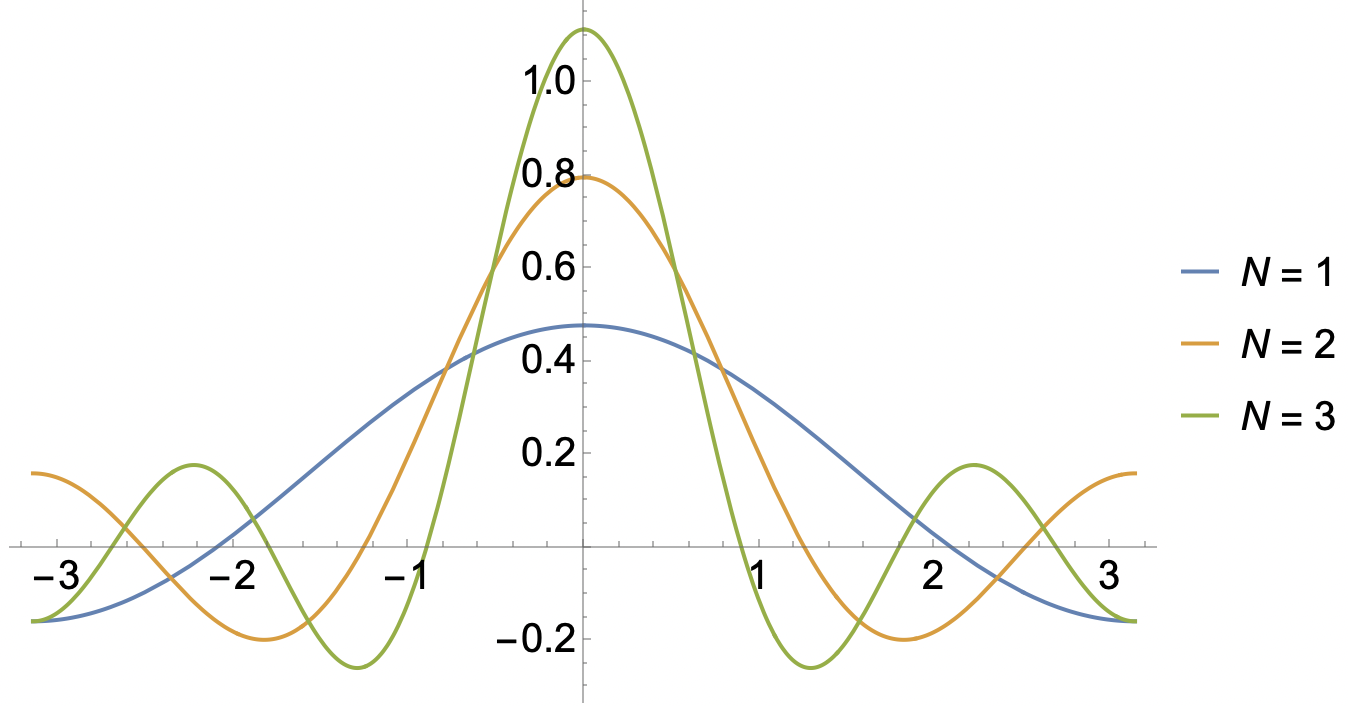
\includegraphics[width=0.6\linewidth]{fig/dirichlet-kernel.png}
  \caption{Plot of Dirichlet kernel $D_N(x)$ on $[-\pi, \pi]$
  for $N = 1,2,3$.}
  \label{dirichlet-kernel}
\end{figure}

\begin{proof}
If $f \in L^2([- \pi, \pi])$, we have 
\[
\begin{aligned}
S_N f(x) 
&= \sum_{\abs{n} \leq N} \left( \frac{1}{2\pi} 
\int_{- \pi}^\pi f(t) e^{- i n t} \d t \right) e^{i n x} \\
&= \int_{-\pi}^\pi f(t) \left( \frac{1}{2\pi} 
\sum_{\abs{n} \leq N} e^{i n (x - t)} \right) \d t.
\end{aligned}
\]
Let $D_N(x) = \frac{1}{2\pi} 
\sum_{\abs{n} \leq N} e^{i n (x - t)}$. 
Then for $x \neq 0$, we have 
\[
\begin{aligned}
  D_N(x) 
  &= \frac{1}{2\pi} \sum_{n=-N}^{N} 
  e^{- i n x} \\ 
  &= \frac{1}{2\pi} e^{- i N x} \sum_{n=0}^{2N}
  \left( e^{i x} \right)^n \\
  &= \frac{1}{2\pi} e^{- i N x} 
  \frac{1 - e^{i (2N+1) x}}{1 - e^{i x}} \\
  &= \frac{1}{2\pi} \frac{e^{i (N + \frac{1}{2}) x} 
  - e^{- i (N + \frac{1}{2}) x}}{e^{\frac{ix}{2}} - 
  e^{-\frac{ix}{2}}} \\
  &= \frac{1}{2\pi} \frac{2 i \sin (N + \frac{1}{2})x}
  {2i \sin \frac{x}{2}} \\
  &= \frac{1}{2\pi} \frac{\sin (N + \frac{1}{2})x}
  {\sin \frac{x}{2}},
\end{aligned}
\]
as desired. For $x = 0$, we also clearly have 
$D_N(0) = \frac{(2N+1)}{2\pi}$. The proof is thus 
complete.
\end{proof}

\begin{defi}
If $f \in L^2([-\pi, \pi])$, we define the 
\textbf{$N$-th Cesaro-Fourier mean} of $f$ by 
\[
\sigma_N f(x) = \frac{1}{N+1} \sum_{k=0}^N 
S_k f(x).
\]
\end{defi}

The idea behind defining the Cesaro mean is that 
if the original sequence converges, the Cesaro mean 
also converge to the same limit. However, Cesaro 
have even better property --- the Cesaro mean 
can converge even if the original sequence does not 
converge. Therefore, it has better convergence properties
and hopefully we can show it converge to $f$ in $L^2$ more 
easily. The goal now is then to show 
\[
\norm{\sigma_N f - f}_2 \to 0 \text{ as $N \to \infty$}.
\]
This would tell us if all Fourier coefficients are zero, 
then the Cesaro means are zero, and the limit above 
would tell us $f$ is zero.

\subsection{Fejer's theorem and convergence 
of Fourier series}

In this section, we will show that if $f \in L^2 ([-\pi, \pi])$,
then $\norm{\sigma_N f - f}_2 \to 0$ as $N \to \infty$.

First we will rewrite the Cesaro Fourier mean, just like 
what we did for the partial Fourier sum using the 
Dirichlet kernel.
\begin{thm}
For any $f \in L^2([-\pi, \pi])$, we have 
\[
\sigma_N f(x) = \int_{-\pi}^\pi K_N(x - t) f(t) \d t,
\]
where 
\[
K_N(x) = \begin{cases}
  \frac{N+1}{2\pi} & (x = 0) \\
  \frac{1}{2\pi (N + 1)} \frac{\sin^2 \frac{N+1}{2}x}
  {\sin^2 \frac{x}{2}} & (x \neq 0)
\end{cases}
\]
is the Fejer kernel.

Moreover, we have 
\begin{enumerate}
  \item $K_N(x) \geq 0$, $K_N(x) = K_N(-x)$, and $K_N(x)$ 
  is $2\pi$ periodic.

  \item $\int_{-\pi}^\pi K_N(t) \d t = 1$.
  
  \item If $\delta \in (0, \pi]$, then for all 
  $\delta \leq \abs{x} \leq \pi$, we have 
  \[
  \abs{K_N(x)} \leq \frac{1}{2\pi (N+1) \sin^2 \frac{\delta}{2}}.
  \]
\end{enumerate}
\end{thm}

A plot for $K_N(x)$ is shown in Figure \ref{fejer-kernel}. 

\begin{figure}[h!]
  \centering
  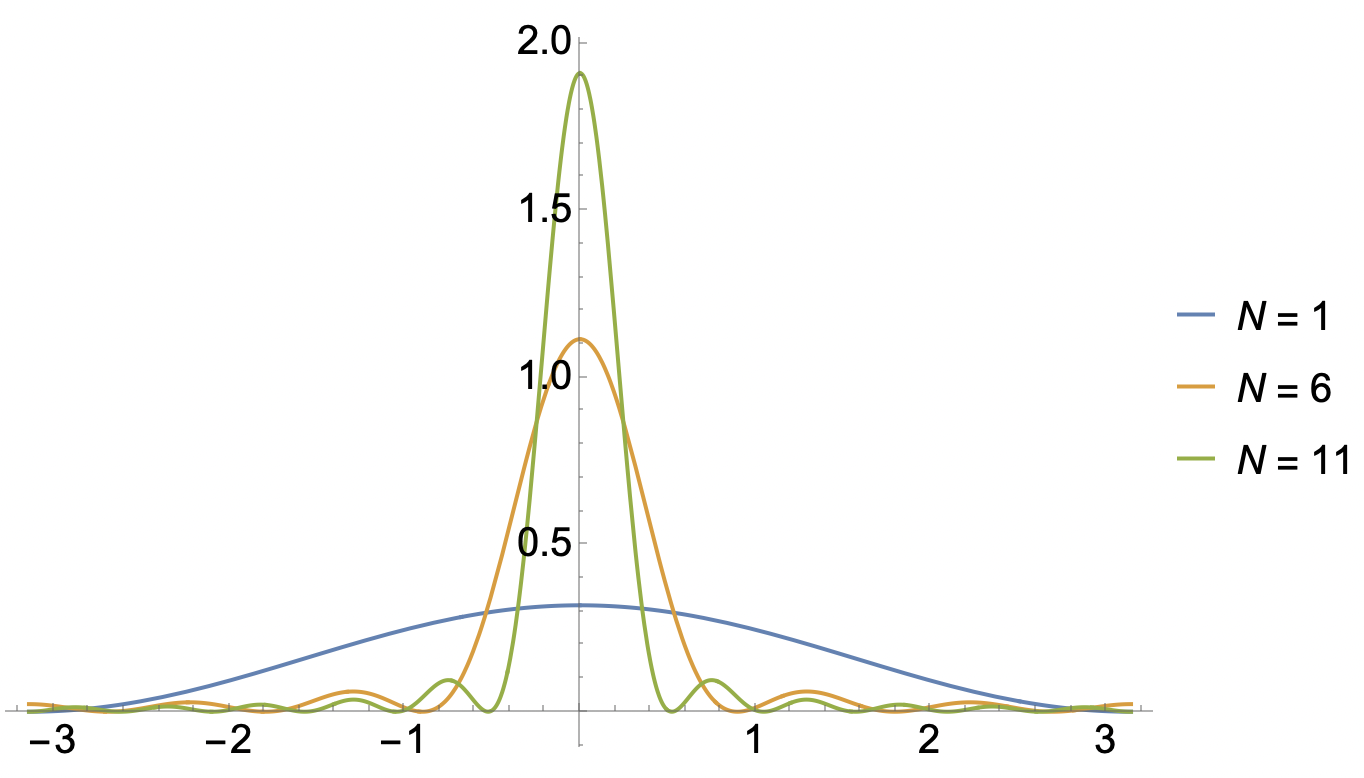
\includegraphics[width=0.6\linewidth]{fig/fejer-kernel.png}
  \caption{Plot of Dirichlet kernel $D_N(x)$ on $[-\pi, \pi]$
  for $N = 1,6,11$.}
  \label{fejer-kernel}
\end{figure}

Note that $K_N(x)$ is concentrated at $0$ 
when $N$ is very large. In this case, we have 
\[
\begin{aligned}
  \sigma_N f(x) 
  &= \int_{-\pi}^\pi K_N(x - t) f(t) \d t \\
  &\approx f(x) \int_{-\pi}^\pi K_N(t) \d t \\
  &= f(x).
\end{aligned}
\]
This provides a rough intuition behind the Fejer kernel. 
The fact that $K_N$ is non-negative makes a huge difference 
compared to the Dirichlet kernel, since it gives much better 
properties.

\begin{proof}
Recall that 
\[
S_k f(x) = \int_{-\pi}^\pi D_k(x - t) f(t) \d t,
\]
where 
\[
D_k(t) = \begin{cases}
  \frac{2 N + 1}{2 \pi} & (t = 0), \\
  \frac{1}{2\pi} \frac{\sin (N + \frac{1}{2})t}{\sin \frac{t}{2}}
  & (t \neq 0).
\end{cases}
\]
It follows that 
\[
\begin{aligned}
  \sigma_N f(x) 
  &= \frac{1}{N+1} \sum_{k=0}^N S_k f(x) \\ 
  &= \int_{-\pi}^\pi \frac{1}{N+1} \sum_{k=0}^N D_k(x - t) f(t) \d t. 
\end{aligned}
\]
Then for $x \neq 0$, we have 
\[
\begin{aligned}
  K_N(x)
  &= \frac{1}{N+1} \sum_{k=0}^N D_k(x) \\
  &= \frac{1}{2\pi (N+1)} \frac{1}{2 \sin^2 \frac{x}{2}} 
  \sum_{k=0}^N 2 \sin \frac{x}{2} \sin \left( k + \frac{1}{2} \right) x \\
  &= \frac{1}{2\pi (N+1)} \frac{1}{2 \sin^2 \frac{x}{2}} 
  \sum_{k=0}^N \left[ \cos k x - \cos(k + 1) x \right] \\ 
  &= \frac{1}{2\pi (N + 1)} \frac{1}{\sin^2 \frac{x}{2}} 
  \frac{1 - \cos(N + 1)}{2} \\
  &= \frac{1}{2\pi (N+1)} \frac{\sin^2 \frac{N+1}{2} x}{\sin^2 
  \frac{x}{2}}.
\end{aligned}
\]

It follows immediately that $K_N(x) \geq 0$, $K_N(x)$ 
is even and $2\pi$ periodic. 

For property 2, 
note that for all $k$,
\[
\int_{-\pi}^\pi D_k(t) \d t 
= \int_{-\pi}^\pi \sum_{n=-k}^k e^{i n t} \d t
= 1.
\]
Then, 
\[
\int_{-\pi}^\pi K_N(t) \d t 
= \frac{1}{N+1} \sum_{k=0}^N \int_{-\pi}^\pi D_k(t) \d t 
= 1,
\]
as desired.

For property 3, let $\delta \in (0, \pi]$. Note that 
$\sin^2 \frac{x}{2}$ is even and increasing on 
$[0, \pi]$. It follows that $\delta \leq \abs{x} \leq \pi$
implies $\sin^2 \frac{x}{2} \geq \sin^2 \frac{\delta}{2}$. 
Therefore,
\[
K_N(x) \leq \frac{1}{2\pi (N+1)} \frac{\sin^2 \frac{N+1}{2}x}
{\sin^2 \frac{\delta}{2}} 
\leq \frac{1}{2 \pi (N+1) \sin^2 \frac{\delta}{2}}.
\]
\end{proof}

Since the continuous functions that vanishes at both end 
points is dense in $L^2([-\pi, \pi])$, it make sense 
to first prove the theorem for continuous functions.
We have the following theorem by Fejer.

\begin{thm}[Fejer]
  If $f \in C([-\pi, \pi])$ is $2\pi$-periodic,
  $f(\pi) = f(-\pi)$, then 
  $\sigma_N f \to f$ uniformly on $[-\pi, \pi]$.
\end{thm}

\begin{proof}
First we extennd $f$ by periodicity to all of $\R$.
Then $f \in C(\R)$, $2\pi$-periodic. This implies that 
$f$ is uniformly continuous and bounded. 

Let $\epsilon > 0$. Since $f$ is uniformly continuous, 
there exists $\delta > 0$ such that $\abs{y - z} < \delta$ 
implies that $\abs{f(y) - f(z)} < \frac{\epsilon}{2}$. 
Choose $M \in \N$ such that
\[
\frac{2 \norm{f}_\infty}{(N+1) \sin^2 \frac{\delta}{2}} 
< \frac{\epsilon}{2}.
\]
for all $N \geq M$. 
Also, since $f$ and $K_N$ are both $2\pi$-periodic,
we have 
\[
\begin{aligned}
  \sigma_N f(x) 
  = \int_{-\pi}^\pi K_N(x - t) f(t) \d t 
  = \int_{x - \pi}^{x + \pi} K_N(\tau) f(x - \tau) \d \tau 
  = \int_{-\pi}^{\pi} K_N(\tau) f(x - \tau) \d \tau.
\end{aligned}
\]
Then for all $N \geq M$ and for all $x \in [-\pi, \pi]$,
we have 
\[
\begin{aligned}
\abs{\sigma_N f(x) - f(x)} 
&= \abs{\int_{-\pi}^\pi K_N(t) f(x-t) \d t - 
\int_\pi^\pi K_N(t) f(x) \d t} \\
&\leq \int_{-\pi}^\pi K_N(t) \abs{f(x - t) - f(x)} \d t \\
&\leq \int_{\abs{t} < \delta} K_N(t) \abs{f(x - t) - f(x)} \d t
+ \int_{\delta \leq \abs{t} \leq \pi} K_N(t) \abs{f(x - t) - f(x)} \d t \\ 
&\leq \frac{\epsilon}{2} \int_{\abs{t} < \delta} 
K_N(t) \d t + 2 \norm{f}_\infty \int_{\delta \leq \abs{t} \leq \pi}
\frac{1}{2\pi (N+1) \sin^2 \frac{\delta}{2}} \d t \\
&\leq \frac{\epsilon}{2} + \frac{2 \norm{f}_\infty}{(N+1) 
\sin^2 \frac{\delta}{2}} \\
&\leq \epsilon.
\end{aligned}
\]
\end{proof}

\begin{remark}
The same proof can be modified if instead of $K_N(x) \geq 0$,
we have
\[
\sup_{N \in \N} \int_{-\pi}^\pi \abs{K_N(x)} \d x < \infty.
\]
Note that 
\[
\int_{-\pi}^\pi \abs{D_N(x)} \d x \sim \log N,
\]
so we cannot reproduct the proof using Dirichlet kernel.
\end{remark}

We only need some last bit of information to conclude 
the answer of our main question.

\begin{thm}
For all $f \in L^2([-\pi, \pi])$, we have 
$\norm{\sigma_N f}_2 \leq \norm{f}_2$.
\end{thm}

\begin{proof}
Suppose first the $f \in C([-\pi, \pi])$ and $2\pi$-periodic.
Then $\sigma_N f(x) = \int_{-\pi}^{\pi} K_N(t) f(x - t) \d t$.
It follows that 
\[
\begin{aligned}
  \int_{-\pi}^\pi \abs{\sigma_N f(x)}^2 \d x
  &= \int_{-\pi}^\pi \int_{-\pi}^{\pi}
  \int_{-\pi}^{\pi} f(x - s) \bar{f(x - t)} K_N(s) K_N(t) 
  \d s \d t \d x \\
  &= \int_{-\pi}^{\pi} \int_{-\pi}^{\pi} K_N(s) 
  K_N(t) \left[ \int_{-\pi}^{\pi} f(x - s) 
  \bar{f(x - t)} \d x \right] \d s \d t \\
  &\leq \int_{-\pi}^{\pi} \int_{-\pi}^{\pi} 
  K_N(s) K_N(t) \norm{f(\cdot - s)}_2 \norm{f(\cdot - t)}_2 
  \d s \d t \\
  &\leq \norm{f}_2^2 \int_{-\pi}^{\pi} \int_{-\pi}^{\pi} 
  K_N(s) K_N(t) \d s \d t \\
  &= \norm{f}_2,
\end{aligned}
\]
where we used Cauchy-Schwarz inequality. 
This implies that $\norm{\sigma_N f}_2 \leq \norm{f}_2$.

Now for the general case, by density there exists 
sequence $\seqinfn{f_n}$ of $2\pi$-periodic continuous 
function that $\norm{f_n - f}_2 \to 0$. Then, 
$\norm{\sigma_N f_n - \sigma_N f} \to 0$
as $n \to \infty$. Therefore, 
\[
\norm{\sigma_N f}_2 = \lim_{n \to \infty} \norm{\sigma_N f_n}_2 
\leq \lim_{n \to \infty} \norm{f_n}_2 = \norm{f}_2.
\]
\end{proof}

\begin{thm}
For all $f \in L^2([-\pi, \pi])$, we have 
$\norm{\sigma_N f - f}_2 \to 0$ as $N \to \infty$. 
In particular, as a immediate corollary, 
if $\hat{f}(n) = 0$ for all $n \in \Z$, 
then $f = 0$.
\end{thm}

\begin{proof}
Let $f \in L^2([-\pi, \pi])$ and $\epsilon > 0$. 
Again by density there exists $g \in C([-\pi, \pi])$
$2\pi$-periodic such that $\norm{f - g}_2 \leq
\frac{\epsilon}{3}$. Since $\sigma_N g \to g$ uniformly
on $[-\pi, \pi]$, there exists $M \in \N$ such that 
for all $N \geq M$ and all $x \in [-\pi, \pi]$, we have 
\[
\abs{\sigma_N g(x) - g(x)} < \frac{\epsilon}{3 \sqrt{2 \pi}}.
\]
Then for all $N \geq M$, 
\[
\begin{aligned}
\norm{\sigma_N f - f}_2 
&\leq \norm{\sigma_N (f - g)}_2 + \norm{\sigma_N g - g} 
+ \norm{g - f}_2 \\
&\leq 2 \norm{f - g}_2 + \left( \int_{-\pi}^{\pi} \abs{\sigma_N g(x)
- g(x)}^2 \d x \right)^{\frac{1}{2}} \\
&\leq \epsilon.
\end{aligned}
\]
\end{proof}

\begin{remark}
We have shown that for all $f \in L^2([-\pi, \pi])$,
$\norm{S_N f - f}_2 \to 0$. This does not say $S_N f$ 
converge to $f$ almost everywhere. However, by a theorem 
by Carleson, for all $f \in L^2([-\pi, \pi])$, 
we actually do have $S_N f \to f$ almost everywhere.
Also, for all $1 < p < \infty$, $\norm{S_N f - f}_p \to 0$.
This is not true for $p = 1$ or $p = \infty$.
\end{remark}

\subsection{Minimizers, orthogonal complements, and the 
Riesz representation theorem}

\end{document}